\documentclass{article}
\usepackage[utf8]{inputenc}
\usepackage{mathtools}
\usepackage{amsmath}
\usepackage{amssymb}
\usepackage{witharrows}
\usepackage{cancel}
\newcommand{\norm}[1]{\left\lVert#1\right\rVert}

\title{Deep Learning}
\author{Pietro Marcatti}
\date{First Semester 2022/2023}

\begin{document}

\maketitle
\section{History of Deep Learning}
\subsection{Perceptron}
The perceptron algorithm was invented in 1958. The perceptron became the first model for binary classification. It has one weight $w_i$ per input $x_i$. If the result is larger than a threshold it returns 1 otherwise 0 or -1 (non linearity ?).
To train a perceptron we repeat the following steps:
\begin{itemize}
    \item Initialize weigths randomly
    \item Take one sample $x_i$ and predict $y_i$
    \item For erroneous predictions update weights
    \begin{itemize}
        \item If prediction $y = 0$ and ground truth $y_i$ = 1, increase the weights
        \item If prediction $y = 1$ and ground truth $y_i$ = 0, decrease the weights
    \end{itemize}
    \item Repeat until no errors are made
\end{itemize}
However the perceptron can't solve a simple, although non-linear, problem such as the XOR. 
To improve on the perceptron model you must add new layers but there was a stagnation on the neural networks research. The stagnation was caused by a lack of motivation from the community due to the discouraging results of the first perceptron models. 
Still during the AI winter a couple important findings were published such as back-propagation and recurrent neural networks.\\\\
In 2009 the ImageNet dataset was published. It colleted images for each of the 100k terms in WordNet (16M images in total). Terms were organized hierearchally, es: Vehicle \textrightarrow Ambulance.
The ImageNet challange was instituted: 1 million images, 1000 classes, top-5 and top-1 error measured. To build ImageNet they started colleting candidate images from the internet. They then classified the candidates with Amazon Mechanical Turk service.\\
A more recent important achievement was the one obtained by AlphaGo a deep learning model, based on reinforced learning, that in 2016 defeated the best Go player.\\
Deep learning is the first class of learning algorithms that is scalable: performance just keeps getting better as you feed them more data. Instead when working on a small amount of data the performance of a traditional learning model (logistic regression, SVM, decision tree etc) is better.\\
The three key factors for deep learning scaling are:
\begin{itemize}
    \item Data
    \item Computation/hardware
    \item Algorithms
\end{itemize}

\section{Logistic Regression}
Let's start with a simple two feature model:
\begin{itemize}
    \item $x_1$ number of lectures you attend
    \item $x_2$ hours spent on the laboratory activities
\end{itemize}
With logistic regression we want to learn a probabilistic function:
$$\hat{y} = P(y=1|x)$$
In particular the goal is to find the parameters $w$ and $b$ of the following function (hypothesis).
$$H_{w,b}(x)= g =(w^T\cdot x+b) = \frac{1}{1+e^{-(w^T\cdot x+b)}}$$
where $g(z)$ is the sigmoid function so that:
$$\begin{cases}
    H_{w,b}(x) >= 0.5 & \text{if } y=1\\
    H_w,b(x)<0.5 & \text{if } y=0
\end{cases}$$
To get our discrete classification we map the output of the hypthesis function as follow:
$$\begin{cases}
    H_{w,b}(x) >= 0.5 & \text{\textrightarrow "1"}\\
    H_w,b(x)<0.5 & \text{\textrightarrow "0"}
\end{cases}$$
The decision boundary is $H_{w,b}(x) = 0.5 \rightarrow w^T\cdot x+b=0\rightarrow-3+x_1+2x_2$ supposing we have $b=3$ and $w=[1,2]$. The hypotesis function is $>0.5$ when the argument is $>0$, that is becuause of the shape and output of the sigmoid.

\subsection{Cost Function}
To find $w$ and $b$ so that:
$$\begin{cases}
    H_{w,b}(x) >= 0.5 & \text{if } y=1\\
    H_w,b(x)<0.5 & \text{if } y=0
\end{cases}$$
the logistic classifirer defines the following cost function:
\begin{equation}
    J(w,b) = \frac{1}{m}\cdot \sum_{i=1}^{m}{Cost(h_{w,b}(x^i),y^i)}
\end{equation}
\begin{equation}
    Cost(h_{w,b}(x^i),y^i)= -y^i\cdot ln(h_{w,b}(x^i))-(1-y^i)\cdot ln(1-h_{w,b}(x^i))
\end{equation}
This cost function or loss function is convex and is derivable respect to $w$ and $b$
In general we call the function to learn the \textbf{hypotesis} but in deep learning it's also called \textbf{model}, the \textbf{cost function} in deep learning is also called \textbf{loss function}.\\\\
Why is random initialization of weights is important? If we used 0 the first hidden layer would all be 0, because we multiplied all inputs for 0.\\
This results that the partial derivates for all nodes in the hidden layers are equal, this is called the symmetry problem.\\\\
We divide our training data set into smaller batches of usually around 16-32-64 samples. We compute forward and backwards on every single sample. Once we complete all the batches we completed an epoch. We can then start again but now, on the first batch, our neural network will have weights that will have already changed thanks to all other batches

\subsubsection*{Regularization}
Logistic Regression: Minimization problem with regularization:$ \;\min_{w,b}{J(w,b)}$
$$J(w,b)= \frac{1}{m}\left[ \sum_{i=1}^{m}{Cost(h_{w,b}(x^{(i)}), y^{(i)})+\frac{\lambda}{2}\sum_{j=1}^{n}{w_i^2}} \right]$$
$\lambda$ is called the regularization parameter, usually b is ignored in the regularization process.
By setting a big regularization parameter we are saying that our minimization algorithm should focus on reducing the weights. The goal is to have the weights all in the same order of magnitude.\\\\
Doesn't regularization kill the importance of some features over others?\\\\
Regularization with Neural Networks:\\
$$J(W^{[1]}, b^{[1]}W^{[2]}, b^{[2]})= \frac{1}{m}\left[ \sum_{i=1}^{m}{\mathbb{L}(\hat{y}, y^{(i)})+\frac{\lambda}{2}\sum_{i=1}^{L}{\norm{W^{[l]}}^2_F}} \right]$$

Where $\lambda$ is the regularization parameter, l is the layer. $$\norm{W^{[i]}}^2_F=\sum_{i=1}^{n{[l-1]}}{\sum_{j=1}^{n^{[l]}}{(W_{i,j}^{[l]})^2}}$$
Where $W^{[l]}\in \mathbb{R}^{n^{[l]}\times n^{[l-1]}}$\\
Regularization helps preventing overfitting because by using a big value for $\lambda$ we minimize weigths close to 0 and some of them are basically dead (almost 0)\\\\
Too many dead nodes means underfitting? Would it ever be useful to have a small $\lambda$\\\\


\subsection*{Normalization}
Mean normalization transforms dta to have a mean of zero and a standard deviation of 1. Such normalization is the preferred normalization for Neural Networks. Given a feature $ x_i $ the mapped feature is $ x^i  = \frac{x_i-\mu_i}{\sigma_i}$ where $ \mu_i, \sigma_i $ are the mean and standard deviation computed on the training set. It is important to normalize each feature separately as its data come from different distributions and the feature number is exactly what the index $ x_i $ refers to.\\
The MinMaxNormalization shifts the data such that all features are exactly between 0 and 1. 
\[ 
    x_{i}^{'}= \frac{x_i-\min{x}}{\max{x} - \min{x}} 
\]
It's very important to apply the same transformation to the trainin set and the test set for the supervised model to work on the test set. The figure illustrates what would happen if we were to use the minimum and range of the test set instead.
\begin{figure}[htbp]
    \centering
    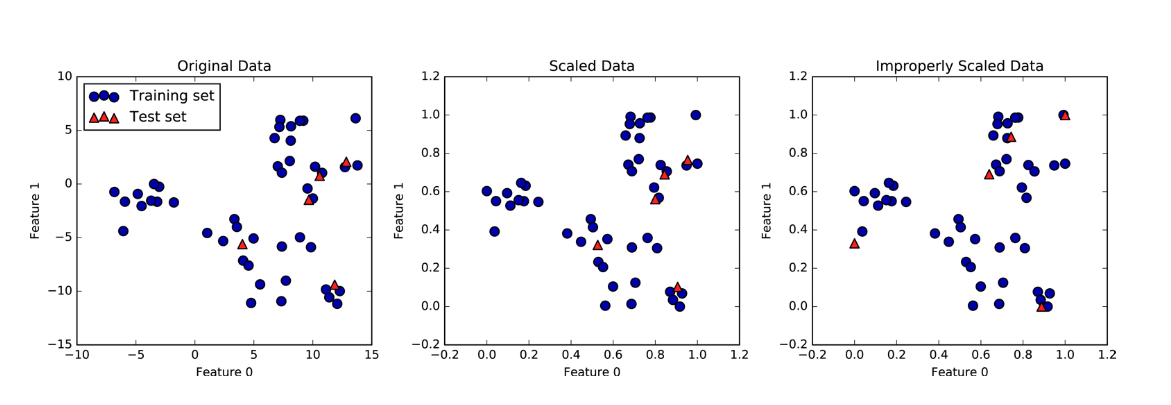
\includegraphics[width=13cm]{normalization-effect.png}
\end{figure}
The correct procedure is to normalize the training set and then once we have a stable model we can normalize also the test set with the same min and max values computed for the training set.

\section*{NLP and Word Embedding}
Natural language processing is a field of deep learning in which you focus on recognizing elements of written text speech particles. Other fields of use are the summarization of text, question answering, automatic email response and forwarding, chatbots ecc ecc\\
Word embedding is a field of deep learning. It aims to represent a word as feature vectors, and consequently as numbers. The simplest way is to assign each word of a vocabulary a number but this way you could sort words which doesn't map as a semantic characterstic for words. A different way is to use a one-hot vector for each words. These vectors are the size of the vocabulary and only for the word we want to represent we put 0 in the corresponding position, otherwise 0. This representation has some pros: it's simple and it doesnt imply ordering. The cons: huge vectors and no embedded meaning. 
\end{document}
